\subsection{Wagasci module}

\begin{figure}[tbh]
\begin{center}
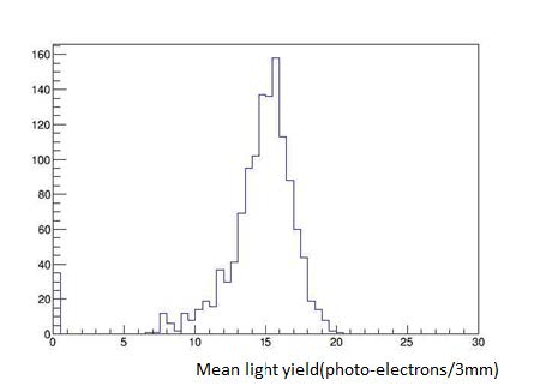
\includegraphics[width=0.5\linewidth]{fig/wmlight.pdf}
\end{center}
\caption{Average light yield for muons produced by the interaction of neutrinos
  in the hall wall.
}
\label{fig:wmlight}
\end{figure}

\begin{figure}[tbh]
  \begin{center}
   \begin{subfigure}{0.48\textwidth}
     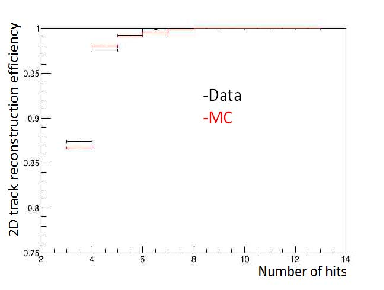
\includegraphics[width=\linewidth]{fig/wmeffvshit.pdf}
    \end{subfigure}
  \begin{subfigure}{0.48\textwidth}
      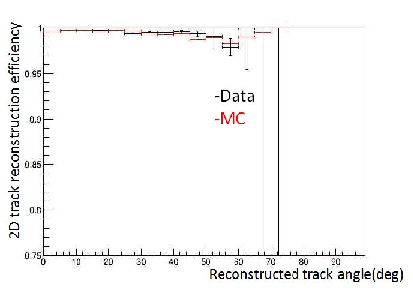
\includegraphics[width=\linewidth]{fig/wmeffvsangle.pdf}
    \end{subfigure}    
    \end{center}
  \caption{2D track reconstruction efficiency as a function of number of hits (left) and track angle (right).}
\label{fig:wmefficiency}
\end{figure}
